\question
Император Палпатин решил задействовать вас в разработке чертежей новой станции "Звезда Смерти 2". Из-за увеличенных размеров она требует ещё лучшей системы коридоров для эффективного перемещения персонала, поэтому в этот раз вам необходимо доработать схему так, чтобы граф состоял из наименьшего числа компонент вершинной двусвязности и стал Эйлеровым. Не забывайте, что даже Имперские ресурсы ограничены, поэтому вам запрещается добавлять новые вершины в граф, а рёбер нужно использовать как можно меньше. После преобразования посчитайте и укажите количество компонент вершинной двусвязности.

\begin{minipage}[h]{0.45\linewidth}
\center{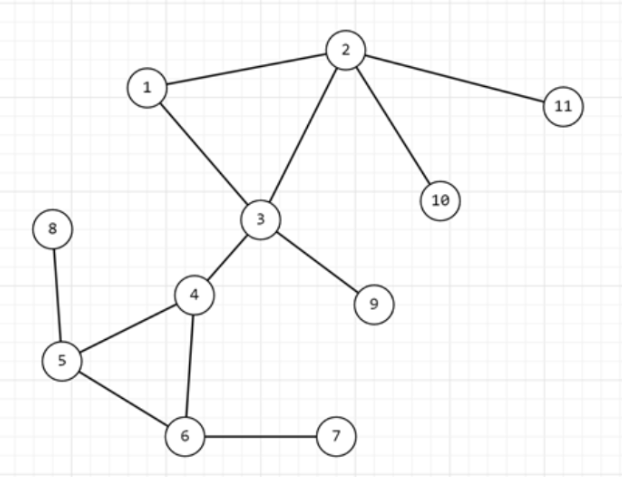
\includegraphics[width=0.7\textwidth]{pic/46.png} }
\end{minipage}

---------------

Автор -- Александр Гущенко, M3303
